\section{Results}
\label{sec:results}

We tested our methods on twenty different $512\times 512$ gray scale images, each with nine different masks of missing pixels. Each mask consisted randomly missing pixels from 10\% to 90\%.

We compare algorithms based on two criteria: the mean-squared error of the original image compared to the reconstructed image and the runtime of the algorithm. The following six inpainting algorithms have been tested:
\begin{enumerate}
	\item Sparse-coding with a DCT dictionary.
	\item Sparse-coding with a learned dictionary.
	\item Singular Value Decomposition.
	\item Regular diffusion with a $K_{\text{diamond}}$ kernel.
	\item Regular diffusion with a $K_{\text{gauss}}$ kernel.
	\item Directional diffusion with patches of size $32 \times 32$.
\end{enumerate}

\begin{figure*}
	\begin{subfigure}[b]{0.48\textwidth}
		\centering
		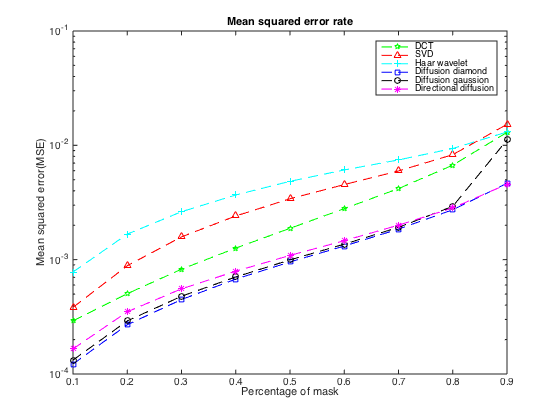
\includegraphics[trim=1.4cm 0.5cm 1.5cm 0.5cm, clip, width=0.9\textwidth]{figures/mse}
		\caption{Mean square error }
		\label{fig:mse}
	\end{subfigure}
	\begin{subfigure}[b]{0.48\textwidth}
		\centering
		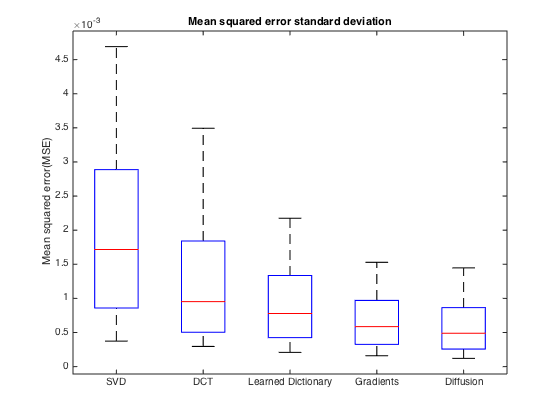
\includegraphics[trim=1.4cm 0.5cm 1.5cm 0.5cm, clip, width=0.9\textwidth]{figures/mse_std}
		\caption{Standard deviation of mean squared error}
		\label{fig:mse_std}	
	\end{subfigure}
\end{figure*}

From figure \ref{fig:err_random} we see that the regular diffusion algorithm with the $K_{\text{diamond}}$ kernel works best on a mask of randomly missing pixels. This phenomenon can be explained by the fact that this algorithm diffuses nearby pixels into the missing regions. On average the randomly missing pixels will have some pixels in its direct or near neighborhood that can be used to infer the pixel value.

Figure \ref{fig:err_text} shows the mean squared error of the algorithms on a fixed mask, namely a piece of text. In this case, the missing pixels have some structure to them and form larger areas of missing pixels. In that case, the directional diffusion algorithm performs best. As the size of the regions of missing pixels gets larger, the regular diffusion algorithm has less nearby pixels to work with. Any high-contrasting edges of the underlying image are not properly extended into the unknown regions. The directional diffusion algorithms helps resolve this by aligning the kernel  $K_{\theta}$ with the general directionality of the image patch. This attempts to propagate high-contrast edges of the image into the unknown regions.


\begin{figure}
		
\end{figure}